%        File: DesignDocument.tex
%     Created: 一 3月 26 01:00 下午 2018 C
% Last Change: 一 3月 26 01:00 下午 2018 C
%
\documentclass[UTF8,noindent]{ctexart}
\usepackage[a4paper,left=2.0cm,right=2.0cm,top=2.0cm,bottom=2.0cm]{geometry}
\usepackage{hyperref}
\usepackage{url}
\usepackage{graphicx}
\usepackage{amsmath}
\usepackage{amssymb}
\usepackage{enumitem}
\usepackage{tikz}
\usepackage{float}
\usepackage{xeCJK}
\usepackage{listings}
\usepackage{xcolor}
\lstset{language = c,numbers=left, showstringspaces=false,keywordstyle= \color{ blue!70 },commentstyle=\color{red!50!green!50!blue!50}, frame=shadowbox, rulesepcolor= \color{ red!20!green!20!blue!20 } 
} 
\CTEXsetup[format={\Large\bfseries}]{section}
\usetikzlibrary{graphs}
%\newtheorem*{lemma}{Lemma}
\title{\CJKfamily{zhkai}计算机网络研讨课实验报告}
\author{{\CJKfamily{zhkai}冯吕}\ $2015K8009929049$}
\date{\today}
\begin{document}
\maketitle
\zihao{5}
\CJKfamily{zhsong}
%\begin{center}
%  \begin{tabular}{|p{15cm}|}
%    \hline
\section{{\CJKfamily{zhhei}实验题目}}网络传输机制实验一
%\hline
\section{{\CJKfamily{zhhei}实验内容}}
在本次实验中,需要实现$TCP$的连接管理:建立连接和关闭连接。

在建立连接的过程中,需要完成三次握手。
\section{{\CJKfamily{zhhei}实验流程}}
\subsection{函数实现}
在本次实验中,首先需要实现连接管理相关函数,需要实现的函数均位于$tcp\_sock.c$和 $tcp\_in.c$两个文件中。

\paragraph{查找函数}
$tcp\_sock.c$中首先需要实现两个查找函数,在$established\ table$和$listen\ table$中查找$socket$。在$established\ table$中查找时,以四元组$hash$,然后进行查找,而在$listen\ table$中进行查找时,只需使用$sport$。

\begin{lstlisting}
struct tcp_sock *tcp_sock_lookup_established(u32 saddr, u32 daddr,
u16 sport, u16 dport)
{
	fprintf(stdout, "TODO: implement this function please.\n");

	int key = tcp_hash_function(saddr, daddr, sport, dport);
	struct tcp_sock *sk_pos, *sk_q;
	list_for_each_entry_safe(sk_pos, sk_q, &
	tcp_established_sock_table[key], hash_list){
		if (saddr == sk_pos->local.ip && daddr == sk_pos->peer.ip \
		&& sport == sk_pos->local.port && dport == sk_pos->peer.port){
			return sk_pos;
		}
	}
	return NULL;
}

struct tcp_sock *tcp_sock_lookup_listen(u32 saddr, u16 sport)
{
	fprintf(stdout, "TODO: implement this function please.\n");
	u8 key = tcp_hash_function(0, 0, sport, 0);
	struct tcp_sock *sk_pos, *sk_q;
	list_for_each_entry_safe(sk_pos, sk_q, &tcp_listen_sock_table[key], 
	hash_list){
		if (sk_pos->local.port == sport){
			struct tcp_sock *child_pos, *child_q;
			list_for_each_entry_safe(child_pos, child_q, 
			&sk_pos->listen_queue, list){
				if (child_pos->local.port == sport 
				&& child_pos->local.ip == saddr){
					return child_pos;
				}
			}
		}
	}
	return NULL;
}
\end{lstlisting}

\paragraph{$tcp\_sock\_connect$函数}
$tcp\_sock\_connect$函数实现主动建立连接。主动建立连接时,四元组已经确定,发送$SYN$数据包,进入$TCP\_SYN\_SENT$状态,然后$wait\_connect$:
\begin{lstlisting}
int tcp_sock_connect(struct tcp_sock *tsk, struct sock_addr *skaddr)
{
	fprintf(stdout, "TODO: implement this function please.\n");
	tsk->peer.ip = ntohl(skaddr->ip);
	tsk->peer.port = ntohs(skaddr->port);
	tsk->local.port = tcp_get_port();
	tsk->local.ip = 0x0a000002;

	tcp_bind_hash(tsk);
	tcp_send_control_packet(tsk, TCP_SYN);
	tcp_set_state(tsk, TCP_SYN_SENT);
	sleep_on(tsk->wait_connect);

	tcp_hash(tsk);

	return -1;
}
\end{lstlisting}

\paragraph{$tcp\_sock\_listen$函数}
该函数设置$socket$的$backlog$,然后进行$TCP\_LISTEN$状态,并将$socket$ \ $hash$到$listen\ table$上:
\begin{lstlisting}
int tcp_sock_listen(struct tcp_sock *tsk, int backlog)
{
	fprintf(stdout, "TODO: implement this function please.\n");
	tsk->backlog = backlog;
	tcp_set_state(tsk, TCP_LISTEN);
	tcp_hash(tsk);
	return 0;
}
\end{lstlisting}

\paragraph{$tcp\_sock\_accept$函数}
该函数实现被动连接的$accept$操作,如果$accept\ queue$不为空,则弹出一个$socket$来服务,否则,$sleep$:
\begin{lstlisting}
struct tcp_sock *tcp_sock_accept(struct tcp_sock *tsk)
{
	fprintf(stdout, "TODO: implement this function please.\n");
	if (!tsk->accept_backlog){
		sleep_on(tsk->wait_accept);
	}
	if (tsk->accept_backlog){
		struct tcp_sock *accept_tsk = tcp_sock_accept_dequeue(tsk);
		tcp_hash(accept_tsk);
		return accept_tsk;
	}
	return NULL;
}
\end{lstlisting}

\paragraph{$tcp\_state\_listen$函数}
该函数处理当处于$TCP\_LISTEN$状态时收到包的操作:首先判断是否为$TCP\_SYN$包,如果是,则分配一个$child\ socket$来服务这个连接请求,然后由$child\ socket$回复$TCP\_SYN\mid TCP\_ACK$包,并将$child\ socket\ hash$到$established\ table$。
\begin{lstlisting}
void tcp_state_listen(struct tcp_sock *tsk, struct tcp_cb *cb, char *packet)
{
	fprintf(stdout, "TODO: implement this function please.\n");
	if (cb->flags & TCP_SYN){
		tsk->local.ip = cb->daddr;
		tsk->local.port = cb->dport;
		struct tcp_sock *child_sock = alloc_tcp_sock();
		child_sock->local.ip = cb->daddr;
		child_sock->local.port = cb->dport;
		child_sock->peer.ip = cb->saddr;
		child_sock->peer.port = cb->sport;
		child_sock->parent = tsk;
		tcp_set_state(child_sock, TCP_SYN_RECV);
		list_add_head(&child_sock->list, &tsk->listen_queue);

		tcp_send_control_packet(child_sock, TCP_SYN | TCP_ACK);
		tcp_hash(child_sock);
	}
	else {
		tcp_send_reset(cb);
	}
}
\end{lstlisting}

\paragraph{$tcp\_state\_syn\_sent$函数}
该函数处理主动建立连接的一方当收到$TCP\_SYN\mid TCP\_ACK$包时的处理:回复$TCP\_ACK$包,然后进行$TCP\_ESTABLISHED$状态,并唤醒$wait\_connect$。
\begin{lstlisting}
void tcp_state_syn_sent(struct tcp_sock *tsk, struct tcp_cb *cb, char *packet)
{
	fprintf(stdout, "TODO: implement this function please.\n");
	if (cb->flags & (TCP_SYN | TCP_ACK)){
		tcp_send_control_packet(tsk, TCP_ACK);
		tcp_set_state(tsk, TCP_ESTABLISHED);
		wake_up(tsk->wait_connect);
	}
	else {
		tcp_send_reset(cb);
	}
}
\end{lstlisting}

\paragraph{$tcp\_state\_syn\_recv$函数}
该函数处理当被动建立连接的一方收到主动建立连接的一方发送过来的$ACK$包时的处理过程:将自身从$parent$的$listen\ queue$移动到$accept\ queue$中,此时,连接已经建立起来了,进入$TCP\_ESTABLISHED$状态。
\begin{lstlisting}
void tcp_state_syn_recv(struct tcp_sock *tsk, struct tcp_cb *cb, char *packet)
{
	fprintf(stdout, "TODO: implement this function please.\n");
	if (cb->flags & TCP_ACK){
		tcp_sock_accept_enqueue(tsk);
		tcp_set_state(tsk, TCP_ESTABLISHED);
		tsk->peer.ip = cb->saddr;
		tsk->peer.port = cb->sport;
		wake_up(tsk->parent->wait_accept);
	}
	else {
		tcp_send_reset(cb);
	}
}
\end{lstlisting}

\paragraph{$tcp\_process$函数}
该函数是处理一个收到包的完整流程,根据$socket$所处的状态和收到包的类型从而进行不同的处理:
\begin{lstlisting}
void tcp_process(struct tcp_sock *tsk, struct tcp_cb *cb, char *packet)
{
	fprintf(stdout, "TODO: implement this function please.\n");
	/*struct tcphdr *tcp_hdr = packet_to_tcp_hdr(packet);*/
	/*struct iphdr *ip_hdr = packet_to_ip_hdr(packet);*/
	if (tsk->state == TCP_CLOSED){
		tcp_state_closed(tsk, cb, packet);
	}

	else if (tsk->state == TCP_LISTEN){
		tcp_state_listen(tsk, cb, packet);
	}

	if (tsk->state == TCP_SYN_SENT){
		tcp_state_syn_sent(tsk, cb, packet);
	}

	else{
		if (!is_tcp_seq_valid(tsk, cb)){
			free(packet);
		}

		else if (cb->flags & TCP_RST){
			if (!tsk->parent){
				tcp_bind_unhash(tsk);
			}
			tcp_set_state(tsk, TCP_CLOSED);
			free_tcp_sock(tsk);
		}

		else if ((cb->flags & TCP_SYN) || (!(cb->flags & TCP_ACK))){
			tcp_send_reset(cb);
			if (!tsk->parent){
				tcp_bind_unhash(tsk);
			}
			tcp_set_state(tsk, TCP_CLOSED);
			free_tcp_sock(tsk);
		}

		else if (cb->flags & TCP_ACK){
			if (cb->flags & TCP_FIN){
				if (tsk->state == TCP_FIN_WAIT_1){
					tcp_send_control_packet(tsk, TCP_ACK);
					tcp_set_state(tsk, TCP_TIME_WAIT);
					tcp_set_timewait_timer(tsk);
				}
				else{
					tcp_set_state(tsk, TCP_CLOSE_WAIT);
					tcp_sock_close(tsk);
				}
			}

			else if (tsk->state == TCP_LAST_ACK){
				if (!tsk->parent){
					tcp_bind_unhash(tsk);
				}
				tcp_set_state(tsk, TCP_CLOSED);
				free_tcp_sock(tsk);
			}

			else {
				tcp_update_window_safe(tsk, cb);
			}
		}
	}
}
\end{lstlisting}

\subsection{运行}
\begin{itemize}
  \item 运行给定网络拓扑:
	\begin{itemize}
	  \item 在节点$h_1$上执行$TCP$程序:执行脚本,禁止协议栈的相关功能,运行服务器模式;
	  \item 在节点$h_2$上执行$TCP$程序:执行脚本,禁止协议栈的相关功能,运行客户端模式,连接至$h_1$,显示建立连接成功后自动关闭连接;
	\end{itemize}
	\item 通过$wireshark$抓包来来验证建立和关闭连接的正确性;
\end{itemize}
\section{{\CJKfamily{zhhei}实验结果}}

运行$TCP$程序之后,能够成功建立连接:
\begin{figure}[H]
  \centering
  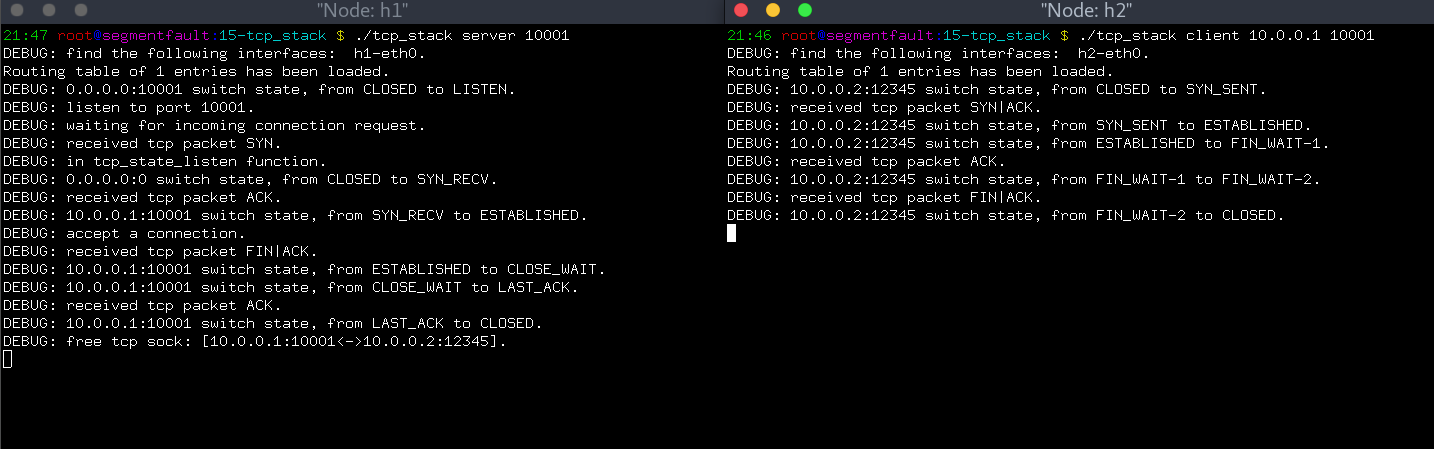
\includegraphics[scale = 0.3]{1.png}
\end{figure}

\section{{\CJKfamily{zhhei}结果分析}}
节点之间能够成功建立$TCP$连接并关闭,实验结果正确。
\end{document}


